% Define document class
\documentclass[twocolumn]{aastex631}
\usepackage{showyourwork}

% \usepackage[dvipsnames]{xcolor}
% \usepackage[colorlinks]{hyperref}
% \usepackage{colortbl}
\definecolor{pyBlue}{RGB}{31, 119, 180}
\definecolor{pyRed}{RGB}{214, 39, 40}
\definecolor{pyGreen}{RGB}{44, 160, 44}

% Link setup
% \newcommand\myshade{80}
% \hypersetup{
%   linkcolor  = pyGreen!\myshade!black,
%   citecolor  = pyBlue!\myshade!black,
%   urlcolor   = pyRed!\myshade!black,
%   colorlinks = true
% }

\newcommand{\jax}{\texttt{JAX}\xspace}
\newcommand{\ripple}{\texttt{ripple}\xspace}
\newcommand{\lalsuite}{\texttt{lalsuite}\xspace}

\newcommand{\TE}[1]{{\color{pyGreen} #1}}
\newcommand{\te}[1]{\textbf{\color{pyGreen}(TE: #1)}}

% Begin!
\begin{document}

% Title
\title{\ripple: Differentiable Waveforms for Gravitational Wave Data Analysis}

\newcommand{\OKC}{\affiliation{The Oskar Klein Centre, Department of Physics, Stockholm University, AlbaNova, SE-106 91 Stockholm, Sweden}} 
\newcommand{\NORDITA}{\affiliation{Nordic Institute for Theoretical Physics (NORDITA), 106 91 Stockholm, Sweden}}
\newcommand{\UdeM}{\affiliation{Département de Physique, Université de Montréal, 1375 Avenue Thérèse-Lavoie-Roux, Montréal, QC H2V 0B3, Canada}} 
\newcommand{\Mila}{\affiliation{Mila -- Quebec AI Institute, 6666 St-Urbain, \#200, Montreal, QC, H2S 3H1}} 
\newcommand{\CGP}{\affiliation{Center for Gravitational Physics, University of Texas at Austin, Austin, TX 78712, USA}}
\newcommand{\CCA}{\affiliation{Center for Computational Astrophysics, Flatiron Institute, New York, NY 10010, USA}}

% Author list
\author{Adam Coogan} \UdeM \Mila
\author{Thomas D.~P.~Edwards} \OKC \NORDITA
\author{Daniel Foreman-Mackey} \CCA
\author{Maximiliano Isi} \CCA
\author{Kelvin Lam} \CCA
\author{Kaze W.~K.~Wong} \CCA
\author{Aaron Zimmerman} \CGP

% Abstract with filler text
\begin{abstract}
    Here we will discuss our implementation of differentiable waveforms and demonstrate their benefits for a variety of data analysis tasks.
\end{abstract}

\section{Introduction}
\label{sec:intro}

% Intro outline
% - What are gravitational waves and what are data analysis tasks?
% - What are derivatives, and how can they be used?
% - What is automatic differentiation, and why has it become particularly useful now? JAX?
% - Discussion of what waveforms are most ameanable to being differentiable
% - In this paper

The discovery of gravitational waves (GWs) from inspiraling and mergering compact objects (COs) has revolutionized our understanding of both fundamental physics and astronomy.
Although the data volumes from GW detectors are relatively small, analyzing the data is a computationally demanding task.
In addition, this computational cost will substatially increase when next generation detectors come online.
The complexity begins before data gathering where one is required to generate banks of template waveforms which will be used for a matched-filter search~\citep{Owen:1998dk, Owen:1995tm}. 
Once potential candidates are found, parameter estimation (PE) is performed to extract the detailed source properties of each event.
In the most minimial example, this requires one to perform MCMC over a 15 dimensional parameter space for each event.
Beyond this simple scenario, more complex waveform models with many additional parameters may be used to test for deviations from General Relativity.
Finally, using the results of the PE, population synthesis models are used to constrain the progenitors systems from which the black holes we see merging today began their journey~\citep{Wong:2022flg}.
All of these tasks require significant compute.
In this paper, we will argue that differentiable waveforms (and more generally differentiable pipelines) can play a significant role in alleaviating this computational demand.

Derivatives are ubiqitously useful throughout data analysis tasks.
For instance, during PE, derivative information can be used to guide the sampling towards regions with higher likelihood values (e.g. in Hamiltonian Monte Carlo~\citep{2017arXiv170102434B} or Gradient Decsent).
This use of gradients is particularly useful for high dimensional spaces.
Unfortunately, in the field of GW data analysis, analytic derivatives of the necessary quantities (such as the likelihood) have historically been difficult to obtain.
Numerical derivatives also suffer from accuracy issues stemming from rounding or truncation errors.
However, recent progress in automatic differentiation (AD) has shown promise in allowing general, fast derivative calcuations for gravitational waveforms~\citep{Coogan:2022qxs}.

Automatic differentiaton is a family of methods used to compute machine precision derivatives with little computational ovearhead. 
AD's recent ascendance is primarily driven by its use in machine learning, particularly for derivative computations of neural networks which use gradient descent during training.
The core idea of AD is that each any mathematical function can be broken down into a small set of basic operations, each with a known differentiation rule.\footnote{
    Of course, non-differentiable functions exist and care must be taken when treating these special cases.
    }
The full derivative can then be contructed using the chain rule.
There are now a variety of AD implementations, most notably in deep learning frameworks such as \texttt{pytorch}~\citep{pytorch} and \texttt{tensorflow}~\citep{tensorflow2015-whitepaper}.
More general frameworks exist in \texttt{julia}~\citep{zygote, forwarddiff}, although \texttt{julia}'s limited use in GW physics precludes its general use.
Here we make use of \jax~\citep{jax2018github} due to its easy integration with \texttt{python} libraries, ability to just-in-time compile, and ability to utilize a variety of computational resources (i.e. CPUs and GPUs) without changes to the code.
\te{Do we need a longer intro to AD here?}

There are a variety of gravitational waveforms currently used in analysis pipelines.
They are generally structured into different families, the most common of which are: the effective one body, the phenomenological inspiral-merger-ringerdown (IMR), and numerical relativity surrogate.
Of these, the phenomenological IMR family is most well suited for an AD implementation in \jax.
In particular, its closed form expression, ... \TE{Why else?}
\te{Do we need more of an intro for why IMRPhenom?}


In this paper we argue that differentiable waveforms will be a vital component for the future of GW data analysis.
In addition, we present \ripple, a small GW \texttt{python} package containing differentiable implementations of some of the main waveforms currently used in LIGO and Virgo analyses. 
The remainder of this paper is structured as follows. 
In Sec.~\ref{sec:waveforms} we discuss the differentiable waveforms implemented in \ripple and perform some benchmarks to demonstrate the speed and accruacy of the derivative calculations. 
In Sec.~\ref{sec:applications} we discuss four distinct applications using differentiable waveforms. 
First, a simple demonstration of accelerated effectualness calculations using gradient descent.
Second, we show that Fisher analyses are quickly enabled using AD.
Third, we implement differnetiable detector response functions and show an illutrative example using Hamiltonian Monte Carlo.
Finally, we illustrate how the fit coefficients that form part of the IMRPhenom waveform models could be improved by high dimensional fitting, enabled by a differentiable waveform. 
The associated code can be found at \ripple~\citep{ripple}.

\section{Differentiable Waveforms}
\label{sec:waveforms}

A variety of waveform families have been developed to accurately model the GW emission from COs. 
When the COs are relatively well separated, the dynamics of the system can be well approximated with post-Newtonian corrections to the... .
However, close to merger, numerical relatively simulations are required to accurately model the GW emission.
Unfortunately, these numerical simulations are computationally expensive and cannot be run in conjunction with data analysis.
Approximate phenomenological waveforms have therefore been constructued to enable relatively fast waveform generation at sufficient accuracy.

The three major waveform families that have been developed to date are: the Effective-one-body (EOB), numerical relativity (NR) surrogate, and phenomenological inspiral-merger-ringdown (PhenomIMR).
Note that unlike NR surrogate, both the EOB and PhenomIMR waveforms are calibrated to NR waveforms.
EOB waveforms require one to model the binary system using a Hamiltonian and are typically slow to evaluate whereas PhenomIMR waveforms are constructed with simple closed-form expressions.
PhenomIMR waveforms are therefore ideally suited for AD, espeically using \jax. 
In this paper we focus mainly on the aligned spin circular orbit model IMRPhenomD~\citep{Husa:2015iqa, Khan:2015jqa}.

The implementation of IMRPhenomD in \lalsuite is mainly in C, and therefore needs to be rewritten natively into \texttt{pyhton} to be compatible with \jax.
We have re-written IMRPhenomD from scratch using a combination of pure \texttt{pyhton} and \jax derivatives.
In addition, we have restructed the code for readability and evaluation speed as well as exposing the internal fitting coefficients to the user (which we will use later in Sec.~\ref{sec:applications}).

To ensure our implempation of IMRPhenomD is faithful to the \lalsuite implementation, we start by defining the noise weighted inner product:
\begin{equation}
    \left(h_{\theta_1}|h_{\theta_2}\right) \equiv 4 \, \mathrm{Re} \int^{\infty}_{0} \mathrm{d} f \, \frac{ h_{\theta_1}(f) h^*_{\theta_2}(f)}{S_n(f)}\, ,
\end{equation}
where $S_n$ is the (one-sided) noise power spectral density (PSD) and $h_{\theta_1}$ is the frequency domain waveform evaluated at the instrinsic parameter point $\theta_1$.
We can then normalize the inner product through
\begin{equation}
    \left[h_{\theta_1}|h_{\theta_2}\right] = \frac{\left(h_{\theta_1}|h_{\theta_2}\right)}{\sqrt{\left(h_{\theta_1}|h_{\theta_1}\right)\left(h_{\theta_2}|h_{\theta_2}\right)}}\, .
\end{equation}
Now we are ready to define the \textit{match} which is given by 
\begin{equation}
    \mathrm{m}(h_{\theta_1}|h_{\theta_2}) \equiv \max_{t_c,\, \phi_c} \left[h_{\theta_1} \, \middle| \, h_{\theta_2} \right]\,
\end{equation}
where $t_c$ and $\phi_c$ are, respectively, the time and phase of coalesence.

Since the match is a measure of the difference between two waveforms, we can use it to demonstrate that the implementation of IMRPhenomD in \ripple accurately matches the \lalsuite implementation.
This is shown in Fig.~\ref{fig:match}, where we have calculated the $\mathrm{m}(h_{\theta_1}|h^{*}_{\theta_1})$ across the entire parameter space.\footnote{
    Specifically, we use 2000 points in the ranges $m_{1,2} = (1,50)\,M_{\odot}$ and $\chi_{1,2} = (-1,1)$. In addition, we evaulated the waveforms on a frequency grid from $32\,$Hz to $1024\,$Hz with frequency spacing $\Delta f = 0.0125 \,$Hz.
}
Here, $h_{\theta_1}$ corresponds to the \ripple waveform implementation and $h^{*}_{\theta_1}$ is the \lalsuite implementation. 
From Fig.~\ref{fig:match}, it is clear that the \ripple waveform matches with the \lalsuite waveform to numerical precision across the majority of the parameter space.
In particular, the blue points indicate parameter points where the $1-\mathrm{m}(h_{\theta_1}|h^{*}_{\theta_1})=0$ and would therefore not appear in the log scale colorbar.
\begin{figure}[ht!]
    \script{random_matches.py}
    \begin{centering}
        \includegraphics[width=\linewidth]{figures/random_matches.pdf}
        \caption{
            This plot should show a match colour bar.
        }
        \label{fig:match}
    \end{centering}
\end{figure}

There remains some slight deviation between the two waveform implementations at higher masses. 
This is likely due to the fact that cubic interpolators, which are used within IMRPhenomD to calculate the ringdown and damping frequencies, are not currently supported in \jax.
Instead, we initially use \texttt{scipy}'s cubic interpolator to create a fine grid of XXX values, which we then linearly interpolate during waveform generation.
Unfortunately, we cannot make the initial cubic interpolation arbitrarily fine as this would add additional computational overhead when loading the data during waveform evaluation.
The remaining error in the waveform at high masses is therefore primarily down to the coarseness in this interpolation.
Note however, that the differences are well below the accuracy requirements of the waveforms and will have no noticeable for realistic data analysis tasks.

For maximum utility, a waveform needs to be fast to evaluate.
Fortunately, the Phenom IMR waveforms are constructed from simple closed form expressions which are therefore computationally efficient.
Since the \lalsuite implementation of IMRPhenomD is written in \texttt{C}, the evaluation of the waveform itself is faster than \ripple.
Benchmarking on a MacBook Pro with an M1 Max Apple Silicon processor, we find that a single waveform evaluation takes $\sim 4\,\mathrm{ms}$ for \lalsuite (interfaced with python) and $\sim 10\,\mathrm{s}$ for \ripple.\footnote{
    For this benchmark we used $16\,\mathrm{Hz}$ and $1024\,\mathrm{Hz}$ for the lowest and highest frequencies respectively. 
    In addition, we used a frequency spacing of $0.0125\,\mathrm{Hz}$. 
    We performed this benchmark by evaluating the waveform $5000$ times and taking the average evaluation time.
}
Although slower on a CPU benchmark, a key advantage of using \jax is its native ability to run on a GPU.
Waveform calls can therefore be evaluated in parallel, massively improving performance. \te{I couldn't get these to be similar on google colab. @Kaze any ideas how to make this fast?}
Generalizing \lalsuite waveforms to run on a GPU would be a significant undertaking.

The primary arguement of this paper is that waveform derivatives will also be invauable to data analysis tasks. 
AD provides two big advantages when it comes to evaluating derivatives compared to numerical differentiation.
Firstly, the accuracy of derivatives from AD are signficantly more stable than finite difference methods.
In particular, finite differences suffer from both rounding and truncation errors, meaning that the user is required to tune the width over which the difference is taken.
On the other hand, AD produces machine precision derivatives with no tuninig.
Secondly, AD scales favourably with the dimensionality of the function.
In particular, for every input dimension, $D$, added one would need to evaluate the function at least $2D$ times to calcuate finite difference derivatives for all input parameters.
For reverse mode AD, one only needs two function calls to evaluate the derivative of all input parameters, regardless of dimenison.\footnote{
    Note that although the number of function calls is small, reverse mode AD does add memory overhead.
    We've not found this to be limiting in any of the situations tested so far.
}
Since the parameter space of GWs in General Relativity (GR) has $\mathcal{O}(10)$ dimensons, the speed of derivative evaluation is less crucial than the stability.
However, this might change for waveforms in beyond GR models where many more parameters are added.

Overall, we have demonstrated that the PhenomIMR waveform family is ideally suited for AD.
Moreover, we have shown that our implementation of IMRPhenomD in \ripple is accurate and quite to evaluate.
In the next section, we will discuss a variety of potential use cases of differentiable waveforms.

% Emphasise the stability of gradients. $Done$
% Not just a faster way of evaluating PhenomD. $Done$
% Change plot to be q vs chieff. $Done$
% Note that lalsuite cannot be made massively parallel on GPUs. $Done$
% Don't need a full section on Fisher, but make sure to mention. People love Fisher.
% Use acceptance rate as a good explanation of speed ups
% Wall time a messy comparison. Based too much off of hardware
% Emphasise that gradients are beneficial

\section{Applications}
\label{sec:applications}

Here, we will illustrate how three core tasks in GW science can be substantially improved through the use of differentiable waveforms.
In the paper we will primarily look at toy examples, leaving a more careful analyses to future work. 
The three tasks discussed here cover a wide range of GW science, starting with waveform development all the way to forecasting and parameter estimation.

\subsection{Fitting Waveform Coefficients}
\label{subsec:hmc}

\te{Kelvin should add stuff here}

\begin{figure}[t]
    \centering
    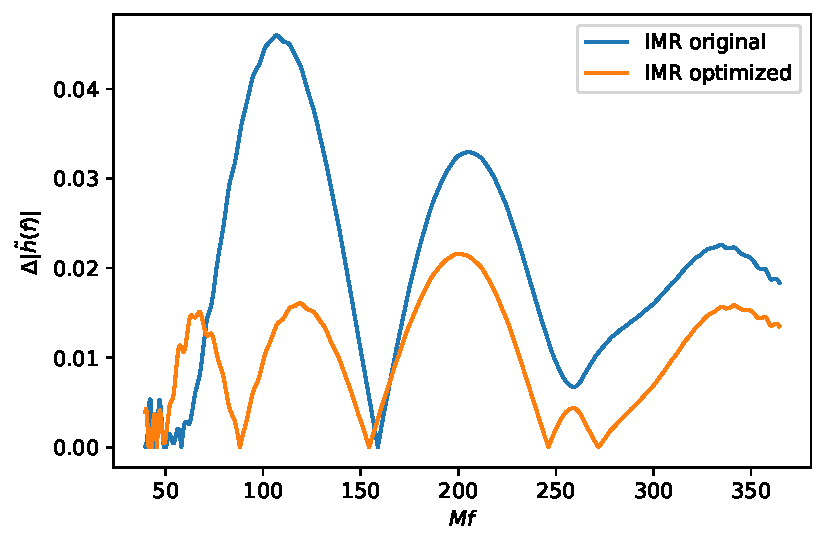
\includegraphics[width=\linewidth]{../static/amplitude_loss.pdf}
    \caption{
        Relative error of amplitudes of IMRPhenomD waveforms. Blue: Error between original Phenom waveform and NR waveform; Orange: Error between optimized waveform and NR waveform.
    }
\end{figure}

\begin{figure}[t]
    \centering
    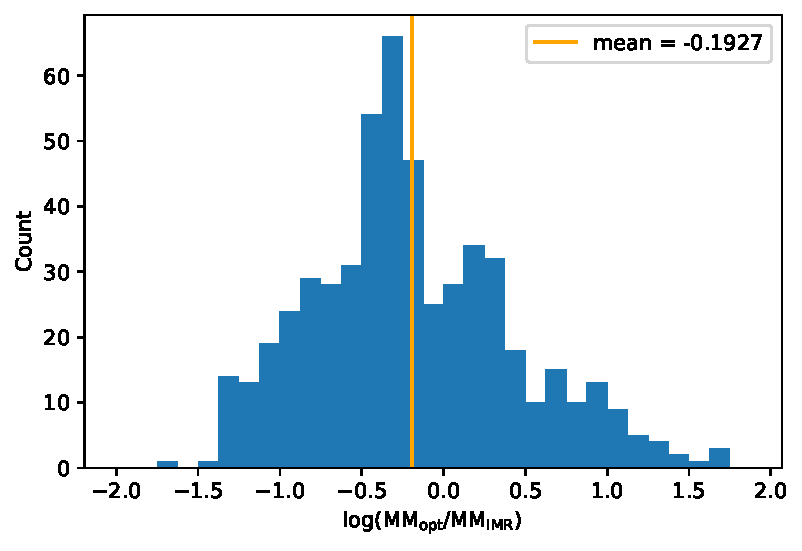
\includegraphics[width=\linewidth]{../static/MM_logdiff_q148.pdf.pdf}
    \caption{
        Distribution of the log difference of mismatches between optimized and original model. The mean shows a 36\% decrease in mismatch. 
    }
\end{figure}



\subsection{Fisher Forecasting}
\label{subsec:hmc}

Forecasting the sensitivity of future experiments is an essential task in GW science.
Due to its theoretical simplicity and its evaluation speed, the Fisher matrix formalism is commonly deployed to estimate how well a binary system's parameters can be measured.
The Fisher matrix approach is built around the assumption of a Gaussian likelihood.
Although in practice this assumption is often violated in real GW datasets, the results obtained using a Fisher analysis can provide quick and useful diagnotistics in evaluating sensitivities for a variety of models and detector configurations.

Computing the Fisher matrix requires one to evaluate derivatives of the likelihhood which in turn involves derivatives of the waveform model and detector projection functions.
AD is therefore perfectly suited for computing Fisher matrices accurately and efficiently. 
Forecasting with Fisher matrices for third generation detectors has already been extensively explored in \citep{Iacovelli:2022bbs, Iacovelli:2022mbg}.
Here we purely want to illustrate the simplicitly and speed of AD for forecasting rather than providing new physics insights.
We therefore consider a simple, three detector setup corresponding to the two LIGO detectors in addition to Virgo.

The Fisher information matrix for a single detector is typically given by 
\begin{equation}
    F^{k}_{ij} = (\partial_i h_0 | \partial_j h_0) \, ,
\end{equation}
where $k$ indicates the detector, $\partial_i = \partial/\partial \theta_i$, and $h_0$ is the strain measured by the detector which is given by,
\begin{equation}
    h_0(\theta) = F_+(\lambda) h_{+}(\phi) + F_\times(\lambda) h_{\times}(\phi) \, .
\end{equation}
Here we have separated out the intrinsic ($\phi$) and extrinsic ($\lambda$) variables.
Since we are considering a three detector setup we simply add the Fisher matrices from the individual detectors to get the combined Fisher matrix:
\begin{equation}
    F_{ij} =  F^{\mathrm{Hanford}}_{ij} + F^{\mathrm{Livingston}}_{ij} + F^{\mathrm{Virgo}}_{ij}   \, .
\end{equation}
Finally, we invert the Fisher matrix to calculate the covariance matrix.

To illustrate the computational speed of computing Fisher matrices with AD, we consider a population of binaries and compute the sky localtization error following Eq.~(28) in \citep{Iacovelli:2022bbs, Iacovelli:2022mbg}.
Since the Fisher matrix approach is known to have both theoretical issues as well as numerical instabilities for low signal-to-noise events, we restrict our population to only nearby systems.
A full list of the distributions used to generate the various parameters in our population are given in Tab...

The distribution of sky localization errors from a a population of $10^3$ binaries can be seen in Fig... 
We have verified that our errors agree with a separate dedicated Fisher forecasting code~\citep{Borhanian:2020ypi} to within X percent.
This demonstrates that AD can be used to accurately produce population level forecasts.

Moreover, each error calculation (including computing the Fisher matrices for each detector and the inversion procress) is substantially faster.
In particular, we find that after compilation each error calculation takes approximately one second on a single computing core.
This can be compared to \texttt{GWbench}~\citep{Borhanian:2020ypi} where each Fisher calculation takes $\mathcal{O}$(minutes) for a similar detector setup and frequency grid.
The factor of almost 60 speed up is despite the fact that a single core evaluation of the \ripple waveform is significantly slower that the \lalsuite call.
As discussed above, performance can be further improved by utilising harware acceleration such as parallel GPU processing.
AD therefore represents a fast and accurate way of performing population level analyses, and should be utilized for testing the capabilities of next generation detectors.

\subsection{Derivative Based Samplers - Hamiltonian Monte Carlo}
\label{subsec:hmc}

\section{Discussion}
\label{subsec:discussion}

\section{Acknowledgments}
This work was supported by collaborative visits funded by the Cosmology and Astroparticle Student and Postdoc Exchange Network (CASPEN).

\bibliography{bib}

\section{Appendix}
\label{sec:appendix}

\end{document}
